


% =============================================================================
% ================================================================ Header Stuff
% =============================================================================

\documentclass{beamer}
\usepackage[utf8]{inputenc}
\usepackage{units} % SI unit typesetting
\usepackage{url} % URL handling
\usepackage{amssymb} % AMS math symbols and helpers
\usepackage{graphicx} % Enhanced graphics support
\usepackage{xspace} % Automatically adjusting space after macros
\usepackage{amsmath} % \text, and other math formatting options
\usepackage{siunitx} % \num{} formatting and SI unit formatting
\usepackage{hyperref} % Add clickable links to other parts of the document
\usepackage{xcolor} % so we can put todo notes in color. 
\usepackage{parskip} % http://ctan.org/pkg/parskip vskip instead of indent. 
\usepackage{float} % Sometimes you want to tell LaTeX to put an image RIGHT HERE. 
\usepackage[percent]{overpic}
\usepackage{beamerthemesplit} % To avoid including backup slides in the page count. 

% Configure the siunitx package
\sisetup{
    group-separator = {,}, % Use , to separate groups of digits, like 12,345
    list-final-separator = {, and } % Always use the serial comma in \SIlist
}

% Input user-defined macros. 


% Highlight an equation (or a section of an equation) in light blue. Make sure,
% if using an align environment, not to have any ampersands inside the
% highlight tag. 
\newcommand{\highlight}[1]{\colorbox{blue!15}{\ensuremath{#1}\xspace}}

\newcommand{\about}{\ensuremath{\sim}}

% This environment is a bulleted list with extra spaces between the entries for legibility. 
\newenvironment{wideitemize}{\itemize\addtolength{\itemsep}{10pt}}{\enditemize}

% Names with special characters. 
\newcommand{\Alfven}{Alfv\'en\xspace}
\newcommand{\Ampere}{Amp\`ere\xspace}
\newcommand{\Schrodinger}{Schr\"odinger\xspace}

% Underline for vectors, double underline for tensors. 
\renewcommand{\vec}[1]{\ensuremath{\underline{#1}}}
\newcommand{\tensor}[1]{\ensuremath{\underline{\underline{#1}}}}

% Differential operators. Make the fractions shorter by using tfrac. 
\newcommand{\dd}[1]{\ensuremath{ \tfrac{\partial}{\partial #1} }\xspace}
\newcommand{\ddt}{\dd{t}\xspace}
\newcommand{\curl}[1]{\ensuremath{ \nabla \times \vec{#1} }\xspace}
\renewcommand{\div}[1]{\ensuremath{ \nabla \cdot \vec{#1} }\xspace}
\newcommand{\grad}[1]{\ensuremath{ \nabla #1 }\xspace}

\newcommand{\dt}{\ensuremath{\delta \hspace{-0.1em} t}\xspace}
\newcommand{\dr}{\ensuremath{\delta \hspace{-0.1em} r}\xspace}
\newcommand{\dL}{\ensuremath{\delta \hspace{-0.1em} L}\xspace}

% Azimuthal modenumber, typically indicated with a lowercase m. 
\newcommand{\azm}{\ensuremath{m}\xspace}

% One over mu zero, in a small fraction. 
\newcommand{\mz}{\ensuremath{\mu_0}\xspace}
\newcommand{\oomz}{\ensuremath{ \tfrac{1}{\mz} }\xspace}



% Define a pair of functions to delimit the backup slides. These ensure that
% they are not counted toward the page count in the bottom corner. 

\newcommand{\backupbegin}{
   \newcounter{finalframe}
   \setcounter{finalframe}{\value{framenumber}}
}
\newcommand{\backupend}{
   \setcounter{framenumber}{\value{finalframe}}
}

% =============================================================================
% ============================================================== Begin Document
% =============================================================================

\title[Short Title]{Long and Descriptive Title}
%\subtitle{PhD Defense}
%\institute{University of Minnesota}
\author{Author Name}
\date{28 April 2016}

% Beamer themes can be perused online. 
\usetheme{Boadilla}
\usefonttheme{serif}

\begin{document}

% =============================================================================
% ================================================================= Title Slide
% =============================================================================

\frame{\titlepage}

% =============================================================================
% ================================================================ Introduction
% =============================================================================

\section{Introduction}

% -----------------------------------------------------------------------------
% -----------------------------------------------------------------------------
% -----------------------------------------------------------------------------

\begin{frame}
\frametitle{Earth's Magnetic Field}

When shaken by the solar wind, etc, Earth's magnetic field lines rattle. 

\vfill

% Image credits can be drawn over an image using the overpic tag. 
\begin{overpic}[width=0.6885\textwidth]{figures/nasa_magnetosphere.jpg}
 \put (0, 1) {\tiny\textcolor{white}{\;NASA}}
\end{overpic}%
\begin{overpic}[width=0.3115\textwidth]{figures/flora_borsi.jpg}
 \put (0, 1) {\tiny\textcolor{white}{\;Fl{\'o}ra Borsi}}
\end{overpic}%

\end{frame}

% =============================================================================
% ======================================================================== Math
% =============================================================================

\section{Math}

% -----------------------------------------------------------------------------
% -----------------------------------------------------------------------------
% -----------------------------------------------------------------------------

\begin{frame}
\frametitle{Maxwell's Equations}

Electric fields are updated using \Ampere's law and Ohm's law:
\begin{align*}
  \tensor{\epsilon} \cdot \ddt \vec{E} = \oomz \curl{B} - \vec{J} - \tensor{\sigma} \cdot \vec{E}
\end{align*}

Let $ \quad \tensor{V}^2 \equiv \oomz \tensor{\epsilon}^{-1} \quad $ and $ \quad \tensor{\Omega} \equiv \tensor{\epsilon}^{-1} \cdot \tensor{\sigma} \quad $ so
\begin{align*}
  \big( \tensor{\Omega} + \tensor{ \mathbb{I} } \ddt \big) \cdot \vec{E} &= \tensor{V}^2 \cdot \big( \curl{B} - \mz \vec{J} \big)
\end{align*}

Which can be solved with an integrating factor: 
\begin{gather*}
  \highlight{\vec{E} \leftarrow \exp \! \big( -\tensor{\Omega} \, \dt \big) \cdot \vec{E} +
    \dt \, \exp \! \big( -\tensor{\Omega} \, \tfrac{\dt}{2} \big) \cdot
    \tensor{V}^2 \cdot \big( \curl{B} - \mz \vec{J} \big) }
\end{gather*}

Magnetic fields are updated using Faraday's law:
\begin{align*}
  \ddt \vec{B} &= -\curl{E} &
  & \text{so} &
  &\highlight{ \vec{B} \leftarrow \vec{B} - \dt \, \curl{E} }
\end{align*}

\end{frame}

% -----------------------------------------------------------------------------
% -----------------------------------------------------------------------------
% -----------------------------------------------------------------------------

% =============================================================================
% ===================================================================== Results
% =============================================================================

\section{Numerical Results}

% -----------------------------------------------------------------------------
% -----------------------------------------------------------------------------
% -----------------------------------------------------------------------------

\begin{frame}
\frametitle{Snapshots of a Low-\azm Simulation}

\begin{wideitemize}
\item Poloidal and compressional waves are blobby. 
\item Toroidal waves are sharply defined. 
\item All components are similar in magnitude. 
\end{wideitemize}

\vfill

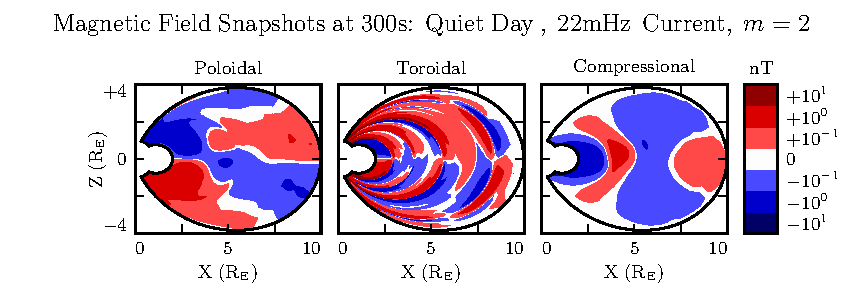
\includegraphics[width=\textwidth]{figures/snapshot_smallm.pdf}

\end{frame}

% =============================================================================
% ================================================================== Conclusion
% =============================================================================

\section{Conclusion}

% -----------------------------------------------------------------------------
% -----------------------------------------------------------------------------
% -----------------------------------------------------------------------------

\begin{frame}
\frametitle{Thanks!}

\begin{columns}
\column{0.33\textwidth}
Committee:
\column{0.34\textwidth}
Funding:
\column{0.33\textwidth}
Collaborators:
\end{columns}

\begin{columns}
\column{0.33\textwidth}
\begin{wideitemize}
\item Bob Lysak (Advisor)
\item Cindy Cattell (Chair)
\item Tom Jones
\item Lindsay Glesener
\end{wideitemize}
\column{0.34\textwidth}
\begin{wideitemize}
\item NSF grant XXXXX
\item UMN OVPR
\item NASA grant YYYYY
\item GEM Student Support
\end{wideitemize}
\column{0.33\textwidth}
\begin{wideitemize}
\item John Wygant
\item Dai Lei
\item Ian Mann
\item Aaron Breneman
\item Scott Thaller
\item Sheng Tian
\end{wideitemize}
\end{columns}

\end{frame}

% =============================================================================
% =============================================================== Backup Slides
% =============================================================================

\backupbegin
\section{Backup Slides}

% -----------------------------------------------------------------------------
% -----------------------------------------------------------------------------
% -----------------------------------------------------------------------------

\begin{frame}
\frametitle{Backup Slide 1}

\end{frame}

% -----------------------------------------------------------------------------
% -----------------------------------------------------------------------------
% -----------------------------------------------------------------------------

\begin{frame}
\frametitle{Backup Slide 2}

\end{frame}

% -----------------------------------------------------------------------------
% -----------------------------------------------------------------------------
% -----------------------------------------------------------------------------

\begin{frame}
\frametitle{Backup Slide 3}

\end{frame}

% =============================================================================
% ================================================================ End Document
% =============================================================================

\backupend

\end{document}



